\subsubsection{\stid{3.13} CLOVER Sub-project PEEKS} \label{subsubsect:peeks}
\paragraph{Overview} 
The PEEKS subproject is a focused team effort to advance the capabilities of the
ECP software stack in terms of communication-avoiding Krylov solvers and
advanced preconditioning techniques featuring fine-grained parallelism.
Previously developed techniques that are available as prototype codes -- as
well as novel algorithm developments -- are turned into production-quality 
implementations and integrated into the ECP software ecosystem 
as part of the Trilinos~\footnote{\url{https://trilinos.org/}} and the  
Ginkgo~\footnote{\url{https://github.com/ginkgo-project/ginkgo}} software 
stacks. 
%With the PEEKS project focus being on algorithm development an software design 
%and leading developers of the Trilinos and Ginkgo software packages being 
%involved in the PEEKS project, a strong focus is on software interoperability 
%and software sustainability. In consequence, there exists a strong link to the 
%other ECP math libraries and the xSDK4ECP project coordinating the ECP 
%mathematical library interoperability efforts. All technology developed in 
%PEEKS is available and disseminated via the xSDK software stack.


\paragraph{Key  Challenges}
Developing preconditioned iterative solvers for the US flagship supercomputers 
deployed in ECP, we acknowledge three major challenges coming from the hardware 
architecture:
\begin{enumerate}
\item 
Fine-grained parallelism in a single node that has to be exploited efficiently 
by the iterative solver and the preconditioner.
\item
Rising communication and synchronization cost as the
computational power is growing much faster than memory power, resulting in 
increased pressure on the bandwidth of all cache/memory levels.
\end{enumerate}

All challenges require the redesign of existing iterative solvers with respect 
to higher parallelism, % within all building blocks
a reduced number of 
communication and synchronization points, favoring computations over 
communication, and adopting multiprecision algorithms for efficient hardware 
utilization. 

\paragraph{Solution Strategy}

The primary thrusts of the PEEKS project are:
\begin{enumerate}
    \item \textbf{Architecture-portable software design:}
	In the Ginkgo C++ software~\cite{anzt2020ginkgo}, we design and develop a 
	next-generation 
	sparse linear algebra library able to run on multi- and manycore 
	architectures. The library design decouples
	algorithm implementations from hardware-specific kernel implementations, 
	thereby acknowledging the importance of platform portability and allowing 
	for extensibility as well as architecture-specific kernel optimization. 
   \item \textbf{Sustainability efforts:}
	The Ginkgo and Trilinos software development adheres the Better Scientific 
	Software (BSSw) design principles~\cite{betterscientificsoftware} that 
	ensure production-quality code by featuring unit testing, automated 
	configuration and installation, Doxygen code documentation, as well as a 
	continuous integration and continuous benchmarking 
	framework~\cite{pasc_anzt}. Ginkgo and Trilinos are 
	open source effort licensed under BSD 3-clause and included in the xSDK and 
	I4S software packages.
   \item \textbf{Pipelined and CA Krylov methods:} 
    	We realize pipelined and 
	communication-avoiding Krylov methods in production-quality code, and 
	we are actively collaborating with the ECP ExaWind project to integrate 
        our new features into their application~\cite{Yamazaki-lowsynch}. 
	\item \textbf{Memory Precision Decoupling:}  In collaboration with the ECP 
	xSDK multiprecision effort, we are working on sparse linear algebra 
	iterative methods and preconditioners that reduce runtime by compressing 
	data before invoking memory operations, such as the adaptive precision 
	block-Jacobi preconditioner~\cite{toms_anzt} and the compressed basis 
	GMRES~\cite{aliaga2020compressed}. 
\end{enumerate}

\paragraph{Recent Progress}
\begin{enumerate}
\item 
The Ginkgo library realized full native support for NVIDIA GPUs (via CUDA) and 
AMD GPUs (via HIP) and became a role model for platform 
portability~\cite{tsai2020preparing}.
\item 
The production-ready implementation of the first parallel threshold ILU 
preconditioner (ParILUT~\cite{ipdps_anzt}) compensates via algorithmic 
improvement for 5 years of hardware development (see 
Figure~\ref{fig:ParILUTperf}).
\item
We implemented and released five variations of communication-avoiding
and pipelined Krylov solvers in the Belos Trilinos package.
\item
We demonstrated the efficient use of communication-avoiding Krylov methods in Trilinos inside wind turbine simulations of the ECP ExaWind 
project~\cite{Yamazaki-lowsynch}.
\item
We developed an initial implementation of a new polynomial preconditioner based on the GMRES polynomial \cite{LoeThornquistBoman20}.
\end{enumerate}

\begin{figure}[htb]
	\centering
	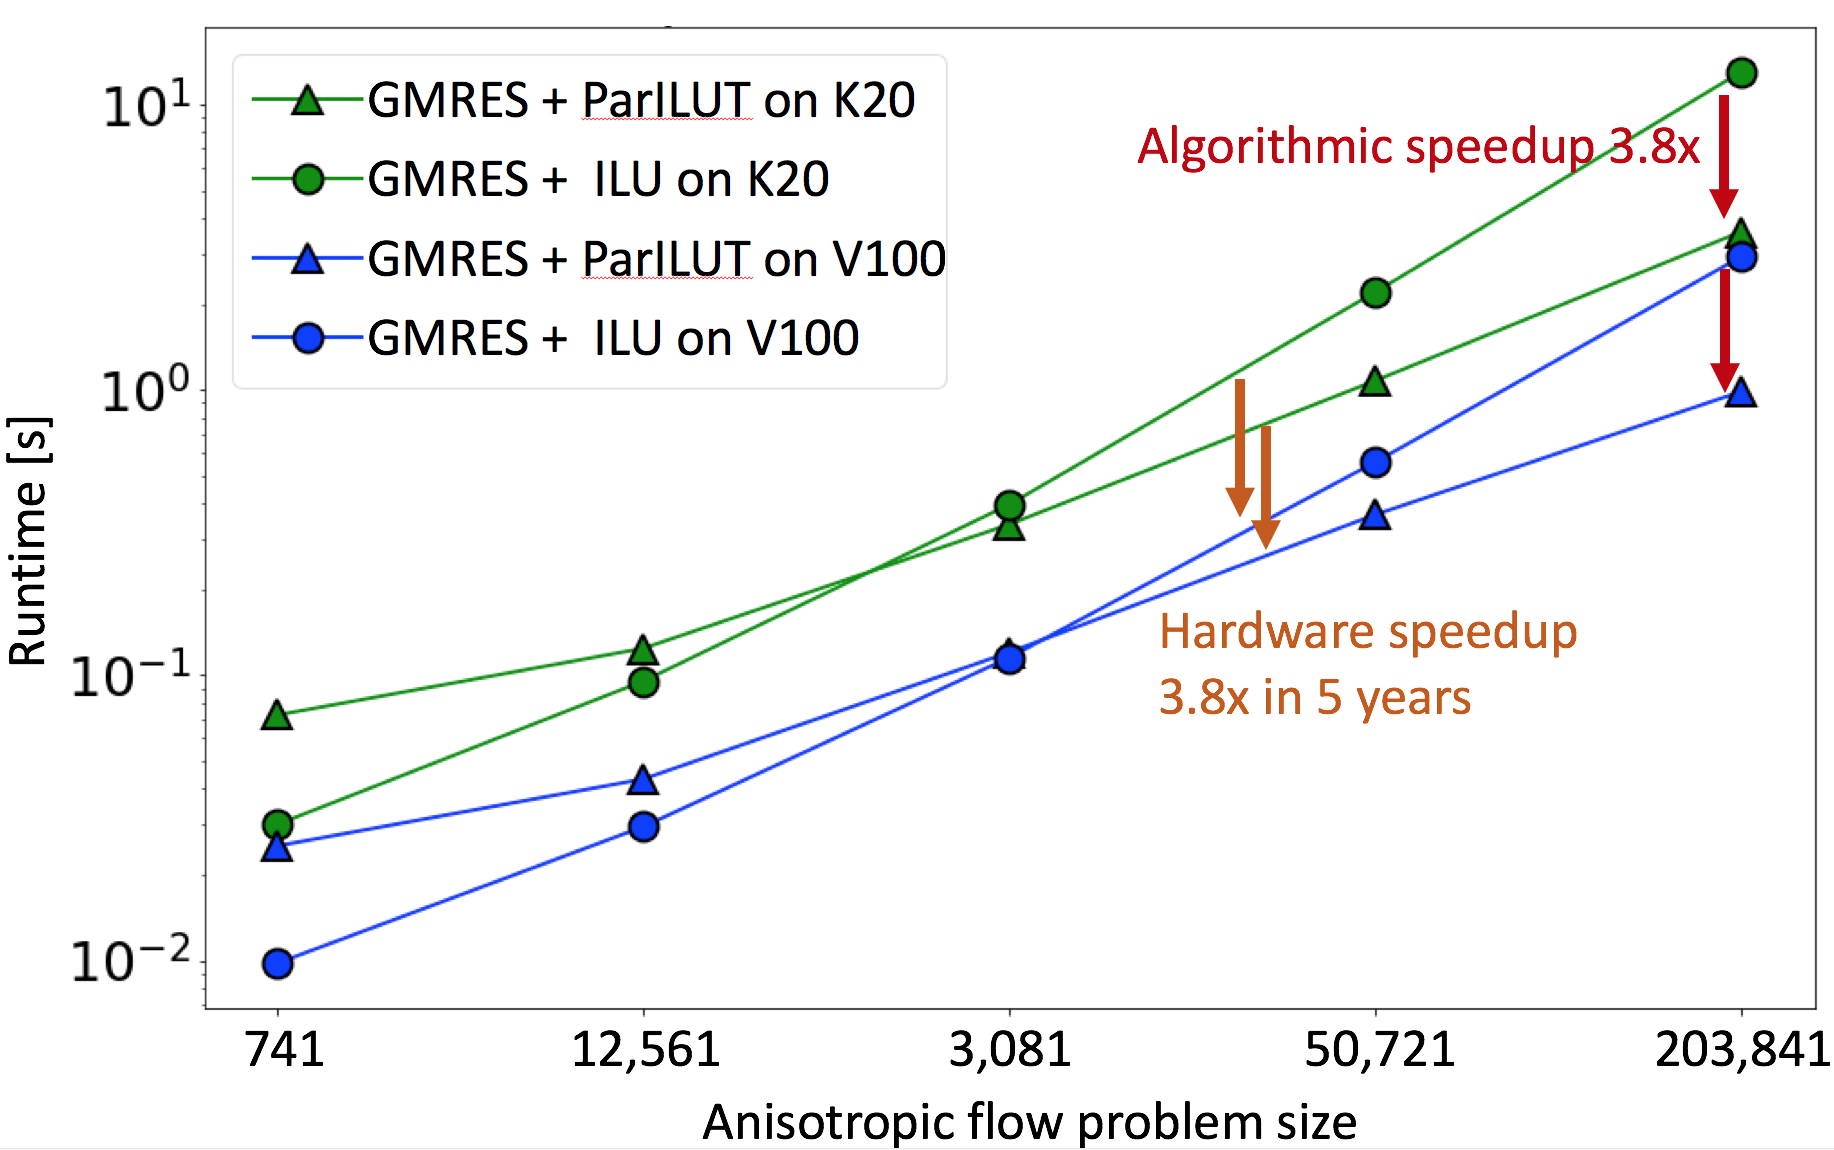
\includegraphics[width=4in]{projects/2.3.3-MathLibs/2.3.3.13-CLOVER/parilut_speedup}
	\caption{\label{fig:ParILUTperf}Time-to-solution performance of anisotropic 
	flow problems of different sizes on different hardware architectures: 
	standard ILU(0) vs. new ParILUT.}
\end{figure}


\paragraph{Next Steps}


Our next efforts are:
\begin{enumerate}
	\item \textbf{Block-versions of the parallel Incomplete factorization 
	preconditioner:} To better reflect the properties of the ECP application 
	projects, we will deploy blocked versions of the ParILU and ParILUT 
	parallel ILU and parallel threshold ILU preconditioners in the Ginkgo 
	software library.
	\item \textbf{Intel GPU backend:} We are currently designing a Ginkgo 
	backend for Intel GPU architectures based on the SYCL language.
	\item \textbf{Compressed Basis Krylov Solvers:} Using the memory accessor 
	designed in the xSDK multiprecision project, we will develop Krylov solvers 
	that reduce the execution time by compressing the Krylov vectors before 
	invoking memory operations.
	\item \textbf{Problem-specific preconditioners for MFEM:} In collaboration 
	with the ECP CEED cluster, we will design problem-specific preconditioners 
	for matrix-free finite element simulations.
	\item \textbf{Low-synchronous orthogonalization:} The success of 
	communication-avoiding Krylov methods motivates to push the synchronization 
	limits further by deploying low-synchronous orthogonalization methods.
        (Collaboration with the ExaWind team at NREL.)
	\item \textbf{Parallel incomplete factorization preconditioner 
	application:} With the advances in the parallel incomplete factorization
	preconditioner generation, the focus increasingly turns to the efficient 
	preconditioner application. We enhance the concept of sparse approximate 
	inverse approximation for incomplete factorization preconditioners, and 
	extend the scope to novel hardware architectures featuring attractive 
	performance in the low-precision regimes.
%	\item \textbf{Get-set usage of software-defined events:} Together with the 
%	Exa-PAPI team, deployed software-defined events (SDE) in the Ginkgo sparse 
%	linear algebra library. These provide the user with access to 
%	domain-specific events like, e.g., preconditioner invocations, 
%	synchronizations, precision format changes. With building blocks differing 
%	in the resource usage, we investigate the possibility of instant power and 
%%	frequency scaling for reducing the power and energy footprint.
%	\item \textbf{Graph analytics kernels:} Preconditioning techniques like 
%	block Jacobi have a strong need for efficient and low-overhead graph 
%	analytics tools identifying strongly-connected components. We deploy GPU 
%	kernels providing this functionality while introducing only negligible 
%	overhead to the preconditioner generation.
	\item \textbf{Polynomial preconditioners:} Polynomial preconditioning is an old idea, but has had limited popularity since it is hard to find good polynomials in the general case. We believe using the GMRES polynomial addresses this issue. Polynomials are also cheap to apply and save communication by reducing the number of inner products. We plan to implement a version using Kokkos that runs on GPU and exascale systems.
\end{enumerate}
